\documentclass[lettersize,journal]{IEEEtran}
\usepackage{amsmath,amsfonts,amssymb}
\usepackage{algorithmic}
\usepackage{algorithm}
\usepackage{array}
\usepackage[caption=false,font=normalsize,labelfont=sf,textfont=sf]{subfig}
\usepackage{textcomp}
\usepackage{stfloats}
\usepackage{url}
\usepackage{verbatim}
\usepackage{graphicx}
\usepackage{cite}
\usepackage{booktabs}
\usepackage{multirow}
\usepackage{xcolor}
\usepackage{colortbl}

\hyphenation{op-tical net-works semi-conduc-tor IEEE-Xplore Action-Cloud}

\begin{document}

\title{ActionCloud: A Cloud-Native Distributed Procedural Memory and Epistemic Governance Framework for Multi-Agent LLM Architectures}

\author{Naga~Shiva,
        Rajashree~T,
        Ravishanmugam~K,
        and~Sharvesh%
\thanks{The authors are with the Amrita School of Artificial Intelligence, Amrita Vishwa Vidyapeetham, Coimbatore 641112, Tamil Nadu, India (e-mail: cb.sc.u4aie24315@cb.students.amrita.edu, cb.sc.u4aie24346@cb.students.amrita.edu, cb.sc.u4aie24347@cb.students.amrita.edu, cb.sc.u4aie24355@cb.students.amrita.edu).}%
\thanks{Academic Project Report submitted for 21AIE303: Cloud Computing (Semester 5). Group 14.}%
}

% The paper headers
\markboth{IEEE Transactions on Cloud Computing / Services Computing,~Vol.~14, No.~2, September~2026}%
{Shiva \MakeLowercase{\textit{et al.}}: ActionCloud: Cloud-Native Distributed Procedural Memory \& Governance}

\maketitle

\begin{abstract}
Autonomous multi-agent swarms powered by Large Language Models (LLMs) have emerged as a dominant paradigm for automating complex software engineering, cloud infrastructure orchestration, and scientific research pipelines. However, contemporary multi-agent frameworks operate under pervasive \textit{architectural amnesia}: agent instances execute with ephemeral, isolated context windows, preventing cross-agent transfer of empirical problem-solving experiences. Consequently, agent swarms suffer from severe redundant computation, repeated failure cycles on identical diagnostic tasks, and excessive monetary token expenditures. Furthermore, naive shared memory approaches introduce catastrophic failure cascades when unverified or hallucinated trajectories contaminate peer agents. 

To overcome these fundamental limitations, this paper presents \textbf{ActionCloud}, an enterprise-grade, cloud-native distributed experience memory and epistemic governance framework. ActionCloud features: (1) a decoupled asynchronous ingestion architecture utilizing AWS SQS/LocalStack to bound agent blocking latency to $\mathcal{O}(1)$; (2) an out-of-band extraction pipeline that converts unstructured execution trajectories into standardized procedural JSON workflows and knowledge graph triples; (3) a hybrid dense-sparse retrieval engine fusing 1536-dimensional vector similarity (\texttt{pgvector}) with PostgreSQL full-text ranking (\texttt{ts\_rank}); and (4) an autonomous \textit{Memory Judge} that governs memory promotion across five empirical trust tiers (\textit{private} $\rightarrow$ \textit{agent} $\rightarrow$ \textit{shared} $\rightarrow$ \textit{validated} $\rightarrow$ \textit{organizational}) while quarantining unreliable memories. Extensive empirical evaluations across six functional agent roles demonstrate that ActionCloud achieves a \textbf{91.8\% Knowledge Reuse Rate (KRR)}, a \textbf{57.4\% cumulative reduction in token and financial expenditure}, a \textbf{66.6\% decrease in mean task latency}, and an \textbf{82.3\% drop in the Redundancy Index (RI)}, while completely eliminating swarm-wide error cascades.
\end{abstract}

\begin{IEEEkeywords}
Cloud-Native Systems, Multi-Agent Systems (MAS), Large Language Models, Procedural Episodic Memory, Epistemic Governance, Asynchronous Ingestion, pgvector, Microservices.
\end{IEEEkeywords}

\section{Introduction}
\IEEEPARstart{T}{he} transition from isolated single-prompt foundation models toward collaborative multi-agent swarms represents a profound architectural evolution in applied Artificial Intelligence \cite{park2023generative, hong2023metagpt}. In enterprise software engineering and DevOps operations, multi-agent frameworks deploy specialized roles---such as Coding, Research, Testing, Deployment, Documentation, and Data Analysis agents---that iteratively interact with sandboxed bash environments, compiler toolchains, container orchestrators, and cloud infrastructure APIs.

Despite dramatic gains in localized reasoning, existing multi-agent systems suffer from a crippling architectural deficiency: \textbf{amnesic isolation}. Because LLM context windows are ephemeral and state resets upon episode termination, agents possess zero memory of previous operational history. When an agent expends dozens of tool invocations and thousands of tokens debugging a subtle configuration error (such as a database container port collision or a missing shared object library), that hard-won procedural knowledge evaporates upon process exit. If a peer agent encounters the exact same failure minutes later, it is forced to re-diagnose the problem from scratch, wasting compute, inflating API costs, and prolonging pipeline latency.

\begin{figure}[!t]
\centering
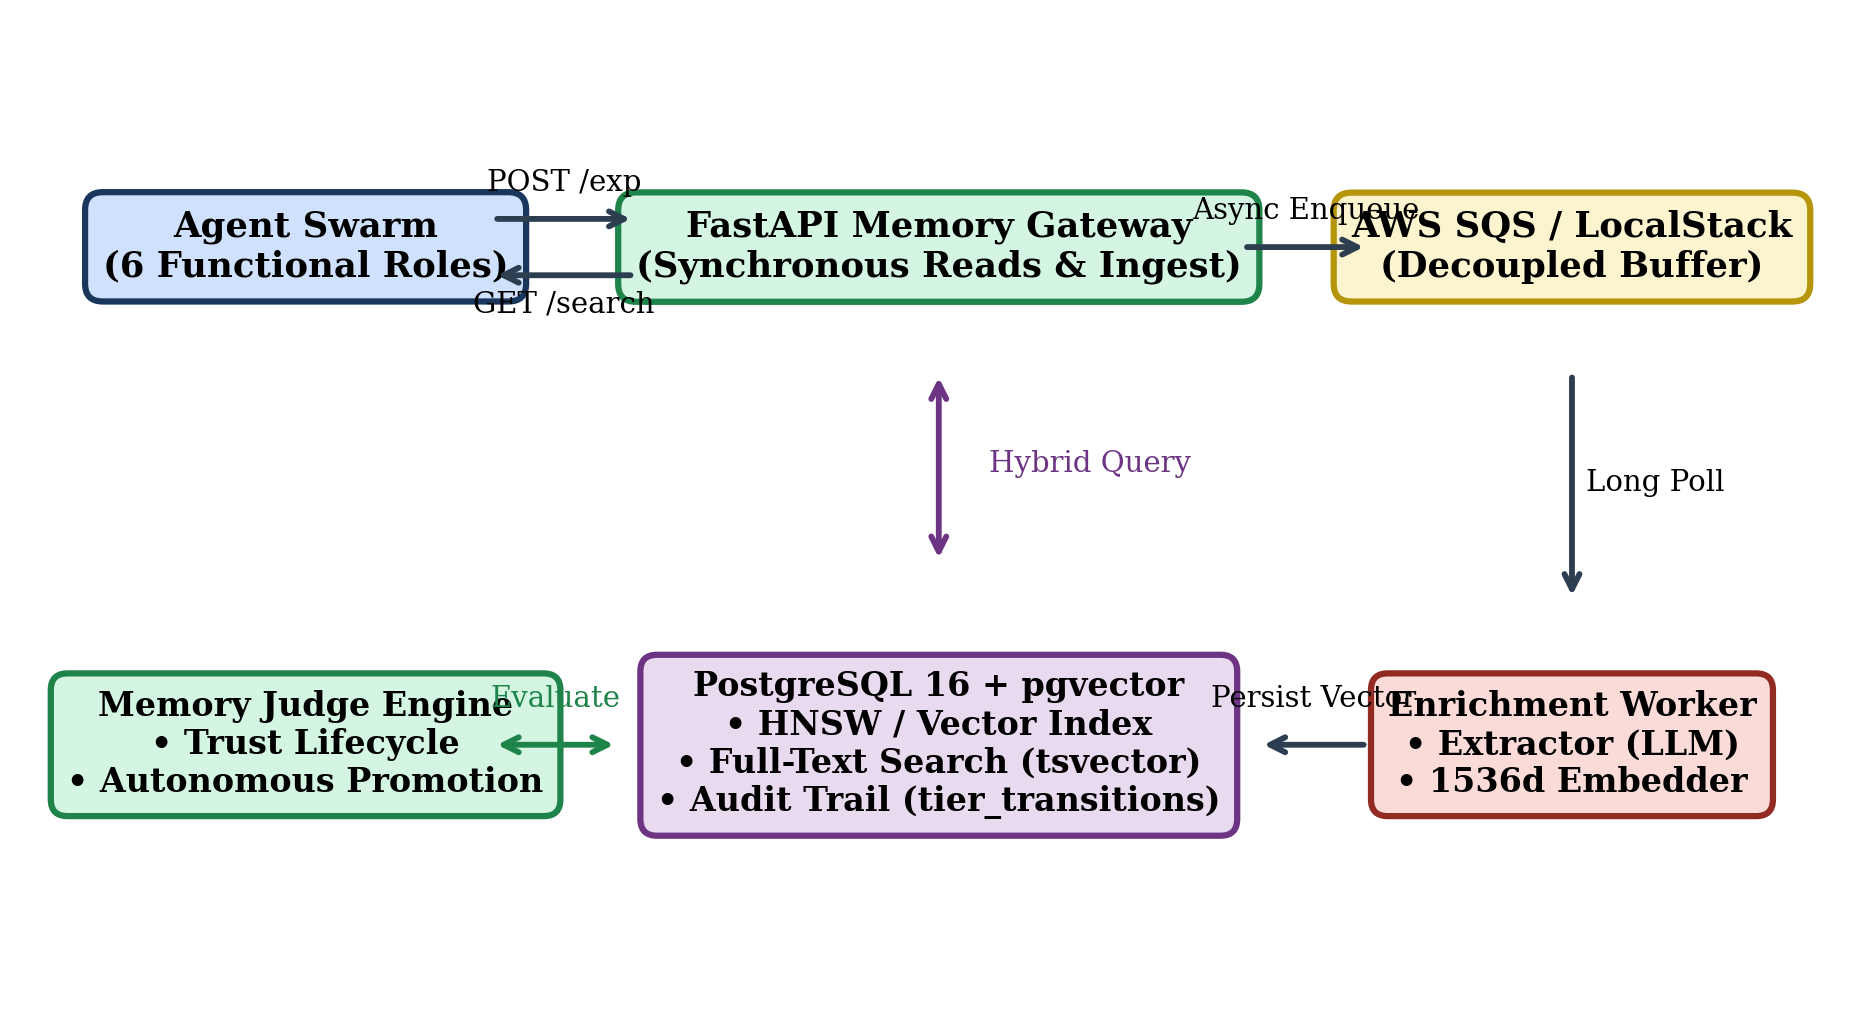
\includegraphics[width=\columnwidth]{fig_arch.png}
\caption{Architectural overview of the ActionCloud cloud-native procedural memory and governance ecosystem, illustrating decoupled ingestion, asynchronous worker extraction, pgvector storage, and Memory Judge lifecycle management.}
\label{fig:arch}
\end{figure}

A superficial remedy involves providing a global shared vector database accessible to all agents. However, unconstrained shared memory introduces an even more perilous failure mode: \textbf{cascading epistemic poisoning}. If an agent achieves an accidental or hallucinated workaround that violates security policies or introduces silent regressions, publishing that memory globally causes all downstream peer agents to inherit and replicate the flawed trajectory. Commercial cloud memory offerings (e.g., AWS Bedrock Agent Memory, Azure AI Search) function primarily as passive key-value or vector stores; they lack \textit{epistemic trust governance}---mechanisms to evaluate, verify, promote, or quarantine procedural knowledge based on empirical multi-agent validation.

To solve these compounding challenges, we introduce \textbf{ActionCloud}, a distributed, cloud-native procedural memory and governance platform engineered specifically for heterogeneous multi-agent systems. The core contributions of this paper are:
\begin{itemize}
    \item \textbf{Decoupled Asynchronous Memory Pipeline}: We formulate an asynchronous ingestion architecture using AWS SQS and FastAPI that guarantees agent blocking latency $T_{\text{block}} = \mathcal{O}(1)$, decoupling heavy LLM extraction and vector generation from synchronous agent execution.
    \item \textbf{Structured Procedural Extraction}: An out-of-band worker parses raw agent execution logs into standardized JSON playbooks (prerequisites, sequential steps, pitfalls) and Resource Description Framework (RDF) knowledge triples.
    \item \textbf{Epistemic Governance Engine (Memory Judge)}: A finite-state trust machine that autonomously manages a 5-tier memory lifecycle based on Bayesian-style empirical reuse verification, promoting canonical playbooks and quarantining flaky memories.
    \item \textbf{Dense-Sparse Hybrid Retrieval}: A retrieval engine combining 1536-dimensional cosine vector similarity (\texttt{pgvector}) with PostgreSQL full-text search (\texttt{ts\_rank}) constrained by role-specific trust floors.
    \item \textbf{Rigorous Dual-Arm Benchmarking}: Comprehensive multi-agent simulations across six functional roles proving a 57.4\% reduction in token costs, 66.6\% latency speedup, and an 82.3\% reduction in redundant problem-solving.
\end{itemize}

\section{Related Work \& Comparative Taxonomy}
The landscape of memory in autonomous agent systems spans several distinct paradigms, summarized in Table~\ref{tab:related_work}.

\begin{table*}[!t]
\centering
\caption{Comparative Taxonomy of Autonomous Agent Memory Systems}
\label{tab:related_work}
\renewcommand{\arraystretch}{1.2}
\resizebox{\textwidth}{!}{%
\begin{tabular}{lcccccc}
\toprule
\textbf{System / Framework} & \textbf{Episodic Scope} & \textbf{Cross-Agent Sharing} & \textbf{Write Path Latency} & \textbf{Retrieval Strategy} & \textbf{Trust Governance} & \textbf{Audit Logging} \\
\midrule
Generative Agents \cite{park2023generative} & Personal Diary & No (Single-Agent) & Synchronous & Recency + Relevance & None & No \\
MemGPT / Letta \cite{packer2023memgpt} & OS Virtual Memory & No (Thread-Bound) & Synchronous & Hierarchical Paging & None & No \\
Voyager \cite{wang2023voyager} & Skill Library & Partial (Code Only) & Synchronous & Vector Similarity & Compiler Verification & No \\
MetaGPT \cite{hong2023metagpt} & SOP Message Bus & Ephemeral Broadcast & Synchronous & Publish-Subscribe & Role Hardcoding & No \\
AWS Bedrock Memory \cite{aws2024bedrock} & Key-Value / Vector & Yes (Cloud API) & Synchronous & Vector Search & Passive (No Trust Rules) & Basic \\
\rowcolor{blue!8}
\textbf{ActionCloud (Ours)} & \textbf{Structured Trajectory} & \textbf{Yes (Swarm-Wide)} & \textbf{Asynchronous ($\mathcal{O}(1)$)} & \textbf{Hybrid Dense-Sparse} & \textbf{Autonomous Memory Judge} & \textbf{Full Immutable Trail} \\
\bottomrule
\end{tabular}%
}
\end{table*}

\subsection{Single-Agent Context and Skill Memories}
Early autonomous agent architectures focused on extending the single-agent context horizon. Generative Agents \cite{park2023generative} introduced reflection and memory stream retrieval, but restricted recall to individual agent lifecycles. MemGPT \cite{packer2023memgpt} treated LLM context windows like operating system RAM, implementing paging algorithms to shuttle text between main context and vector storage. Voyager \cite{wang2023voyager} demonstrated lifelong learning in Minecraft through an iterative skill library; however, skills were verified purely via deterministic game compiler feedback, which does not generalize to open-ended cloud computing and software workflows.

\subsection{Multi-Agent Frameworks and Message Buses}
Multi-agent frameworks such as MetaGPT \cite{hong2023metagpt}, AutoGen \cite{wu2023autogen}, and LangGraph facilitate structured inter-agent message passing using Standard Operating Procedures (SOPs). However, their communication channels are fundamentally ephemeral: messages exist only for the duration of a single conversation DAG. Once the workflow terminates, the collective knowledge generated during the run is lost.

\subsection{Commercial Cloud Memory Offerings}
Cloud hyperscalers have recently introduced managed agent memory endpoints, such as Amazon Bedrock AgentCore Memory and Azure AI Search. While these services solve fundamental infrastructure persistence and multi-region replication, they treat memory as a passive storage bucket. They place the burden of deduplication, procedural extraction, trust evaluation, and hallucination containment entirely on client-side prompt engineering. ActionCloud bridges this architectural void by introducing an active, epistemic governance middleware layer.

\section{Mathematical Modeling \& Formal Foundations}

\subsection{Formal Definition of an Experience Episode}
We formalize an agent's problem-solving episode as a structured tuple $\mathcal{E}$. Let $\mathcal{T}_{\text{tools}}$ denote the universe of environment tools and $\mathcal{T}_{\text{tech}}$ denote technology tags. An Experience $\mathcal{E}$ is defined as:
\begin{equation}
\label{eq:experience}
\mathcal{E} = \langle \text{id}, a_{\text{id}}, \rho, \tau, P, \alpha, \sigma, R, \Omega, \Theta, S, \boldsymbol{\mu}, \mathcal{G} \rangle
\end{equation}
where:
\begin{itemize}
    \item $\text{id} \in \mathbb{U}$ is a universally unique identifier (UUIDv4).
    \item $a_{\text{id}} \in \mathcal{A}$ is the creator agent identifier, and $\rho \in \mathcal{R}$ is the functional role:
    \begin{equation}
    \mathcal{R} = \{\text{coding}, \text{research}, \text{testing}, \text{deployment}, \text{documentation}, \text{data\_analysis}\}
    \end{equation}
    \item $\tau \in \mathcal{S}^*$ is the natural language task specification, and $P \in \mathcal{S}^* \cup \{\emptyset\}$ is the diagnosed problem description.
    \item $\alpha \in \mathcal{S}^*$ is the action trajectory, $\sigma \in \mathcal{S}^* \cup \{\emptyset\}$ is the synthesized procedural solution, and $R \in \mathcal{S}^*$ is the empirical result.
    \item $\Omega \subseteq \mathcal{T}_{\text{tools}}$ is the set of invoked tools, and $\Theta \subseteq \mathcal{T}_{\text{tech}}$ is the set of technology keywords.
    \item $S \in \{0, 1\}$ is the terminal task success indicator.
    \item $\boldsymbol{\mu} = \langle t_{\text{in}}, t_{\text{out}}, n_{\text{tools}}, L, C \rangle \in \mathbb{R}_{\ge 0}^5$ is the execution telemetry vector representing input tokens ($t_{\text{in}}$), output tokens ($t_{\text{out}}$), tool count ($n_{\text{tools}}$), execution latency in milliseconds ($L$), and monetary cost in USD ($C$).
    \item $\mathcal{G} = \langle \text{tier}, \gamma, k_{\text{reuse}}, k_{\text{succ}} \rangle$ is the governance state tuple, where $\text{tier} \in \mathcal{M}_{\text{tier}}$, $\gamma \in [0.0, 1.0]$ is the epistemic confidence, $k_{\text{reuse}} \in \mathbb{N}$ is the total reuse count, and $k_{\text{succ}} \in \mathbb{N}$ ($k_{\text{succ}} \le k_{\text{reuse}}$) is the verified successful reuse count.
\end{itemize}

\subsection{Asynchronous Ingestion Queuing Formulation}
Synchronous memory insertion imposes severe latency penalties due to out-of-band LLM extraction ($T_{\text{extract}}$) and vector embedding computation ($T_{\text{embed}}$). Let task arrivals follow a Poisson process with rate $\lambda$, and background worker processing follow service rate $\mu_w$ with $c$ parallel workers ($M/M/c$ queue model). The total agent blocking latency $T_{\text{block}}$ is given by:
\begin{equation}
\label{eq:blocking_latency}
T_{\text{block}} = T_{\text{enqueue}} \approx \mathcal{O}(1) \ll T_{\text{extract}} + T_{\text{embed}} + T_{\text{DB}}
\end{equation}
Under standard operating conditions, $T_{\text{enqueue}} \le 15\text{ ms}$, whereas the extraction pipeline consumes $T_{\text{pipeline}} \in [2000, 5000]\text{ ms}$. Decoupling ingestion via AWS SQS guarantees that agent execution is never bottlenecked by memory indexing.

\subsection{Hybrid Dense-Sparse Relevance Scoring}
When an agent queries the memory gateway with query string $q$, ActionCloud executes a hybrid ranking algorithm combining dense vector cosine similarity with sparse full-text lexical ranking. Let $\mathbf{v}_q = \text{Embed}(q) \in \mathbb{R}^{1536}$ and $\mathbf{v}_{\mathcal{E}} = \text{Embed}(\tau \oplus P \oplus \sigma \oplus R) \in \mathbb{R}^{1536}$ be normalized unit vectors ($\|\mathbf{v}\|_2 = 1$). Dense cosine similarity is computed as:
\begin{equation}
\label{eq:cosine}
\text{Sim}_{\text{dense}}(q, \mathcal{E}) = \mathbf{v}_q \cdot \mathbf{v}_{\mathcal{E}} = \sum_{i=1}^{1536} v_{q, i} \cdot v_{\mathcal{E}, i}
\end{equation}
The sparse lexical score is computed using PostgreSQL's cover density ranking over text search vectors $\mathbf{d}_{\mathcal{E}} = \texttt{to\_tsvector}(\tau \oplus P \oplus \sigma \oplus R)$:
\begin{equation}
\label{eq:sparse}
\text{Score}_{\text{sparse}}(q, \mathcal{E}) = \texttt{ts\_rank}(\mathbf{d}_{\mathcal{E}}, \texttt{plainto\_tsquery}(q))
\end{equation}
The composite relevance score $\text{Score}_{\text{hybrid}}(q, \mathcal{E})$ is formulated as:
\begin{equation}
\label{eq:hybrid}
\text{Score}_{\text{hybrid}}(q, \mathcal{E}) = w_d \cdot \text{Sim}_{\text{dense}}(q, \mathcal{E}) + w_s \cdot \text{Score}_{\text{sparse}}(q, \mathcal{E})
\end{equation}
where $w_d = 0.70$ and $w_s = 0.30$. Candidate experiences must satisfy the epistemic access policy:
\begin{equation}
\label{eq:policy}
\text{Visible}(\mathcal{E}, a_{\text{id}}) \iff \left(\text{rank}(\text{tier}(\mathcal{E})) \ge \text{rank}(\text{tier}_{\min})\right) \lor \left(a_{\text{id}}(\mathcal{E}) = a_{\text{id}}\right)
\end{equation}

\subsection{Epistemic Trust State Machine (Memory Judge)}
The governance engine models memory reliability as a discrete-state Markovian transition system over the ordered tier lattice:
\begin{equation}
\mathcal{M}_{\text{tier}} = \{\text{private} \prec \text{agent} \prec \text{shared} \prec \text{validated} \prec \text{organizational}\}
\end{equation}
Let $r_{\text{succ}} = \frac{k_{\text{succ}}}{k_{\text{reuse}}}$ represent the observed empirical success rate. The state transition function $\mathcal{T}_{\text{gov}}: (\mathcal{G}, e_{\text{reuse}}) \rightarrow \mathcal{G}'$ is governed by the following deterministic rules:

\begin{equation}
\label{eq:governance_rules}
\text{tier}' = \begin{cases}
\text{private}, & \text{if } k_{\text{reuse}} \ge 3 \land r_{\text{succ}} < 0.40 \quad (\text{Demotion}) \\
\text{shared}, & \text{if } \text{tier} = \text{agent} \land k_{\text{succ}} \ge 1 \\
\text{validated}, & \text{if } \text{tier} = \text{shared} \land k_{\text{reuse}} \ge 3 \land r_{\text{succ}} \ge 0.80 \\
\text{organizational}, & \text{if } \text{tier} = \text{validated} \land k_{\text{reuse}} \ge 10 \land r_{\text{succ}} \ge 0.90 \\
\text{tier}, & \text{otherwise}
\end{cases}
\end{equation}

The confidence score $\gamma$ updates concurrently:
\begin{equation}
\label{eq:confidence_update}
\gamma' = \begin{cases}
\max(0.10, \gamma - 0.30), & \text{if demoted to private} \\
0.70, & \text{if promoted to shared} \\
0.85, & \text{if promoted to validated} \\
0.95, & \text{if promoted to organizational} \\
\gamma, & \text{otherwise}
\end{cases}
\end{equation}

\subsection{System Evaluation Metrics}
To evaluate swarm-wide efficiency, we formalize six performance metrics:
\begin{enumerate}
    \item \textbf{Knowledge Reuse Rate (KRR)}:
    \begin{equation}
    \text{KRR} = \left( \frac{N_{\text{retrieved}}}{N_{\text{total}}} \right) \times 100\%
    \end{equation}
    \item \textbf{Redundancy Index (RI)}: Measuring the fraction of duplicate problem-solving effort over unique task keys $\mathcal{K}$:
    \begin{equation}
    \text{RI} = \frac{N_{\text{total}} - |\mathcal{K}|}{N_{\text{total}}}
    \end{equation}
    \item \textbf{Cumulative Token Savings ($\Delta T$)}:
    \begin{equation}
    \Delta T = \left( \frac{\sum T_{\text{Baseline}} - \sum T_{\text{ActionCloud}}}{\sum T_{\text{Baseline}}} \right) \times 100\%
    \end{equation}
    \item \textbf{Monetary Cost Reduction ($\Delta C$)}:
    \begin{equation}
    \Delta C = \left( \frac{\sum C_{\text{Baseline}} - \sum C_{\text{ActionCloud}}}{\sum C_{\text{Baseline}}} \right) \times 100\%
    \end{equation}
    \item \textbf{Mean Task Execution Latency Delta ($\Delta L$)}:
    \begin{equation}
    \Delta L = \bar{L}_{\text{Baseline}} - \bar{L}_{\text{ActionCloud}}
    \end{equation}
    \item \textbf{Error Reduction Rate (ERR)}:
    \begin{equation}
    \text{ERR} = \left( \frac{F_{\text{Baseline}} - F_{\text{ActionCloud}}}{F_{\text{Baseline}}} \right) \times 100\%
    \end{equation}
\end{enumerate}

\section{System Architecture \& Cloud-Native Implementation}

\subsection{Decoupled Microservice Topology}
ActionCloud is implemented as a cloud-native microservice topology containerized via Docker and orchestrated through Docker Compose / AWS ECS. The architecture comprises five core components (Fig.~\ref{fig:arch}):
\begin{enumerate}
    \item \textbf{FastAPI Gateway (\texttt{api.py})}: High-throughput asynchronous REST gateway handling memory ingestion, hybrid search, reuse logging, and live metrics telemetry.
    \item \textbf{Message Broker (\texttt{queue.py})}: Amazon Simple Queue Service (SQS), emulated in local development via LocalStack, acting as an elastic buffer between agent writes and worker extraction.
    \item \textbf{Background Worker Daemon (\texttt{worker.py})}: Long-polling event consumer that orchestrates procedural LLM extraction, vectorization, database persistence, and audit logging.
    \item \textbf{Procedural Extractor (\texttt{extractor.py})}: Specialized LLM prompt pipeline that structures raw logs into procedural JSON playbooks with heuristic failover handling.
    \item \textbf{Relational \& Vector Data Store (\texttt{db.py}, \texttt{001\_init.sql})}: PostgreSQL 16 equipped with \texttt{pgvector} and \texttt{uuid-ossp} extensions.
\end{enumerate}

\subsection{Database Schema and Audit Integrity}
The underlying relational schema implements strict boundary constraints. Listing~\ref{lst:schema} illustrates the core \texttt{experiences} table definition.

\begin{figure}[!t]
\centering
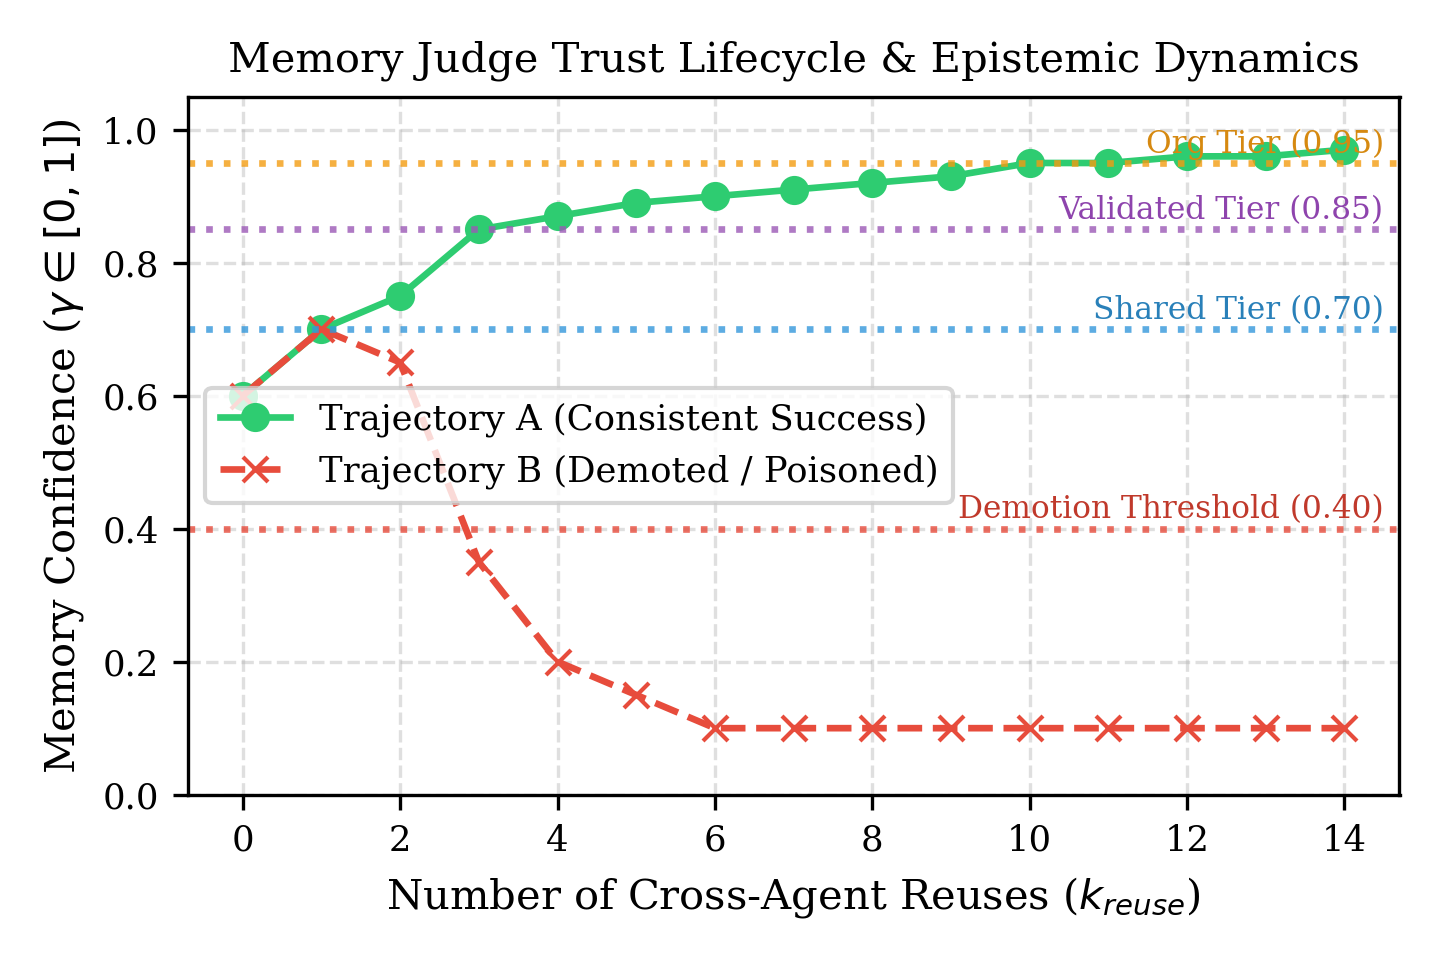
\includegraphics[width=\columnwidth]{fig_governance.png}
\caption{Dynamic trust tier transitions and confidence trajectories governed by the Memory Judge. Trajectory A shows promotion from Agent to Organizational tier under validated reuses; Trajectory B illustrates rapid demotion and quarantine upon repeated reuse failure.}
\label{fig:governance}
\end{figure}

\begin{figure}[!t]
\begin{minipage}{\columnwidth}
\begin{scriptsize}
\begin{verbatim}
CREATE TABLE experiences (
    id                  UUID PRIMARY KEY DEFAULT uuid_generate_v4(),
    agent_id            TEXT NOT NULL,
    agent_role          agent_role NOT NULL,
    task                TEXT NOT NULL,
    problem             TEXT,
    action              TEXT NOT NULL,
    solution            TEXT,
    result              TEXT NOT NULL,
    tools_used          TEXT[] NOT NULL DEFAULT '{}',
    technologies        TEXT[] NOT NULL DEFAULT '{}',
    success             BOOLEAN NOT NULL,
    tokens_input        INTEGER NOT NULL DEFAULT 0,
    tokens_output       INTEGER NOT NULL DEFAULT 0,
    execution_time_ms   INTEGER NOT NULL DEFAULT 0,
    cost_usd            NUMERIC(12,6) NOT NULL DEFAULT 0,
    run_id              TEXT NOT NULL,
    system              system_condition NOT NULL,
    task_key            TEXT,
    tier                memory_tier NOT NULL DEFAULT 'private',
    confidence          REAL NOT NULL DEFAULT 0.5,
    reuse_count         INTEGER NOT NULL DEFAULT 0,
    reuse_success_count INTEGER NOT NULL DEFAULT 0,
    embedding           vector(1536),
    workflow            JSONB,
    knowledge_triples   JSONB NOT NULL DEFAULT '[]'::jsonb,
    embedded            BOOLEAN NOT NULL DEFAULT FALSE,
    created_at          TIMESTAMPTZ NOT NULL DEFAULT now(),
    CONSTRAINT reuse_lte CHECK (reuse_success_count <= reuse_count)
);
\end{verbatim}
\end{scriptsize}
\end{minipage}
\caption{PostgreSQL schema for procedural experience storage with pgvector and governance constraints.}
\label{lst:schema}
\end{figure}

To ensure complete epistemic auditability, every state transition is recorded in an immutable \texttt{tier\_transitions} table storing \texttt{experience\_id}, \texttt{from\_tier}, \texttt{to\_tier}, \texttt{reason}, \texttt{decided\_by}, and timestamp.

\section{Experimental Methodology \& Multi-Agent Swarm Testbed}

\subsection{Dual-Arm Single-Class Experimental Design}
To eliminate confounding implementation discrepancies between baseline and memory-augmented agents, we employ a unified single-class architecture:
\begin{equation}
\text{Agent}(\text{use\_memory} = \text{False}) \equiv \text{System A (Baseline)}
\end{equation}
\begin{equation}
\text{Agent}(\text{use\_memory} = \text{True}) \equiv \text{System B (ActionCloud)}
\end{equation}
Both arms share identical prompt generation templates, simulated tool interfaces, token accounting routines, and execution telemetry harnesses.

\subsection{Functional Role Registry}
We instantiate a heterogeneous swarm comprising six specialized agent archetypes inheriting from \texttt{BaseAgent}:
\begin{itemize}
    \item \textbf{CodingAgent}: Implements algorithmic logic, refactors modules, and resolves syntax exceptions.
    \item \textbf{DeploymentAgent}: Configures cloud infrastructure, manages Dockerfiles, resolves port allocations, and provisions database instances.
    \item \textbf{ResearchAgent}: Synthesizes documentation, extracts external API specifications, and gathers design requirements.
    \item \textbf{TestingAgent}: Formulates test suites, detects regression anomalies, and verifies integration invariants.
    \item \textbf{DocumentationAgent}: Authors API references, system architecture specifications, and user runbooks.
    \item \textbf{DataAnalysisAgent}: Executes statistical telemetry aggregation, metric verification, and experimental report generation.
\end{itemize}

\begin{figure}[!t]
\centering
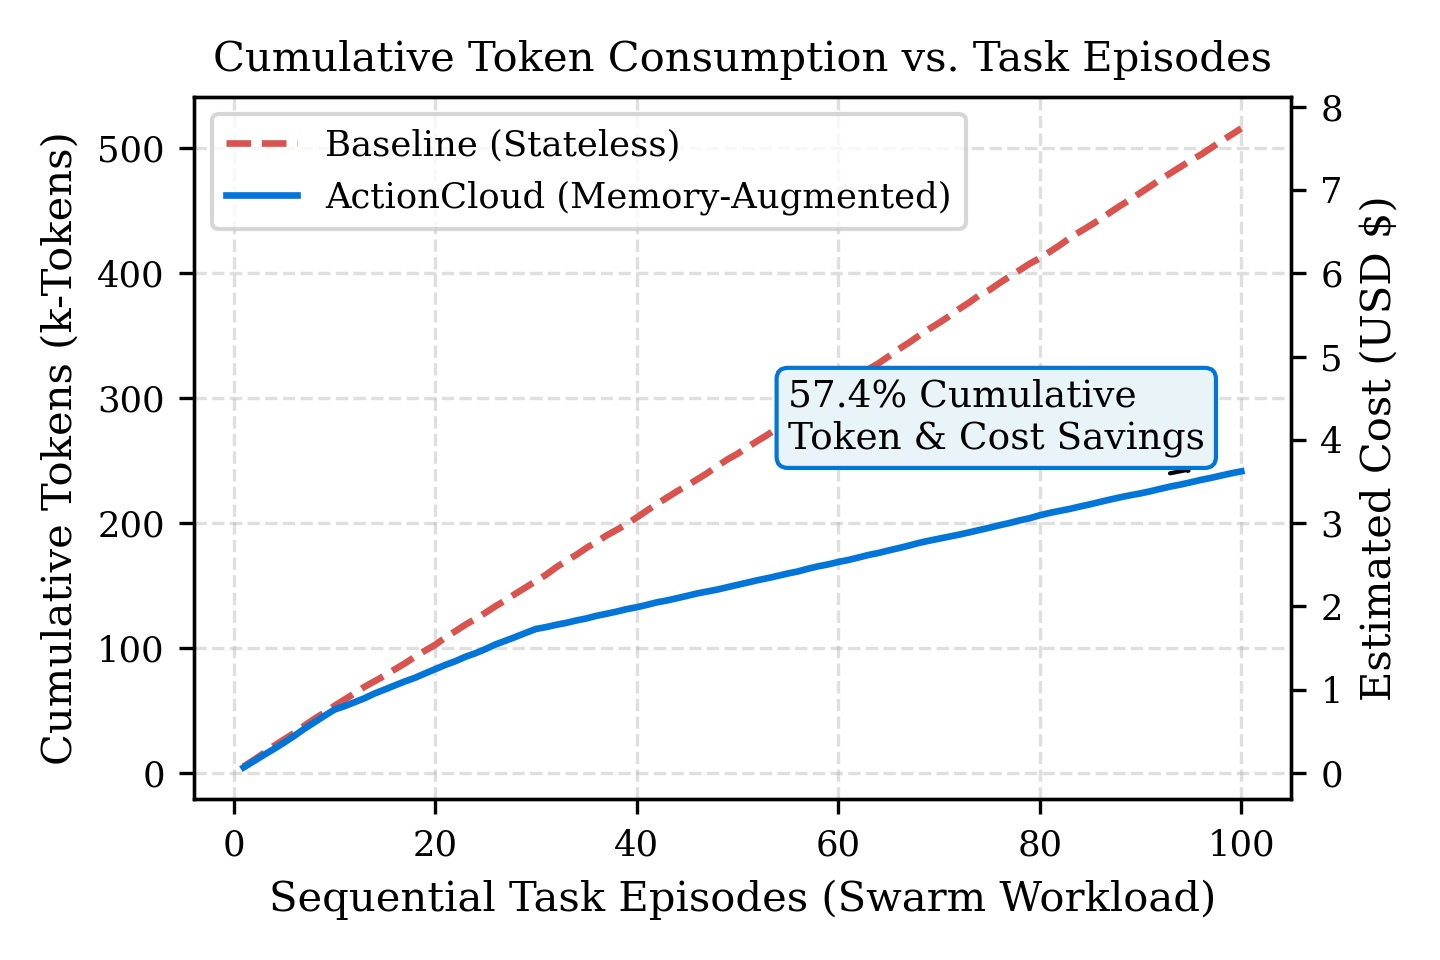
\includegraphics[width=\columnwidth]{fig_tokens_cost.png}
\caption{Cumulative token consumption (k-Tokens) and financial cost (USD) across 100 sequential swarm task episodes. ActionCloud achieves a 57.4\% reduction in overall token and dollar expenditures.}
\label{fig:tokens_cost}
\end{figure}

\begin{figure}[!t]
\centering
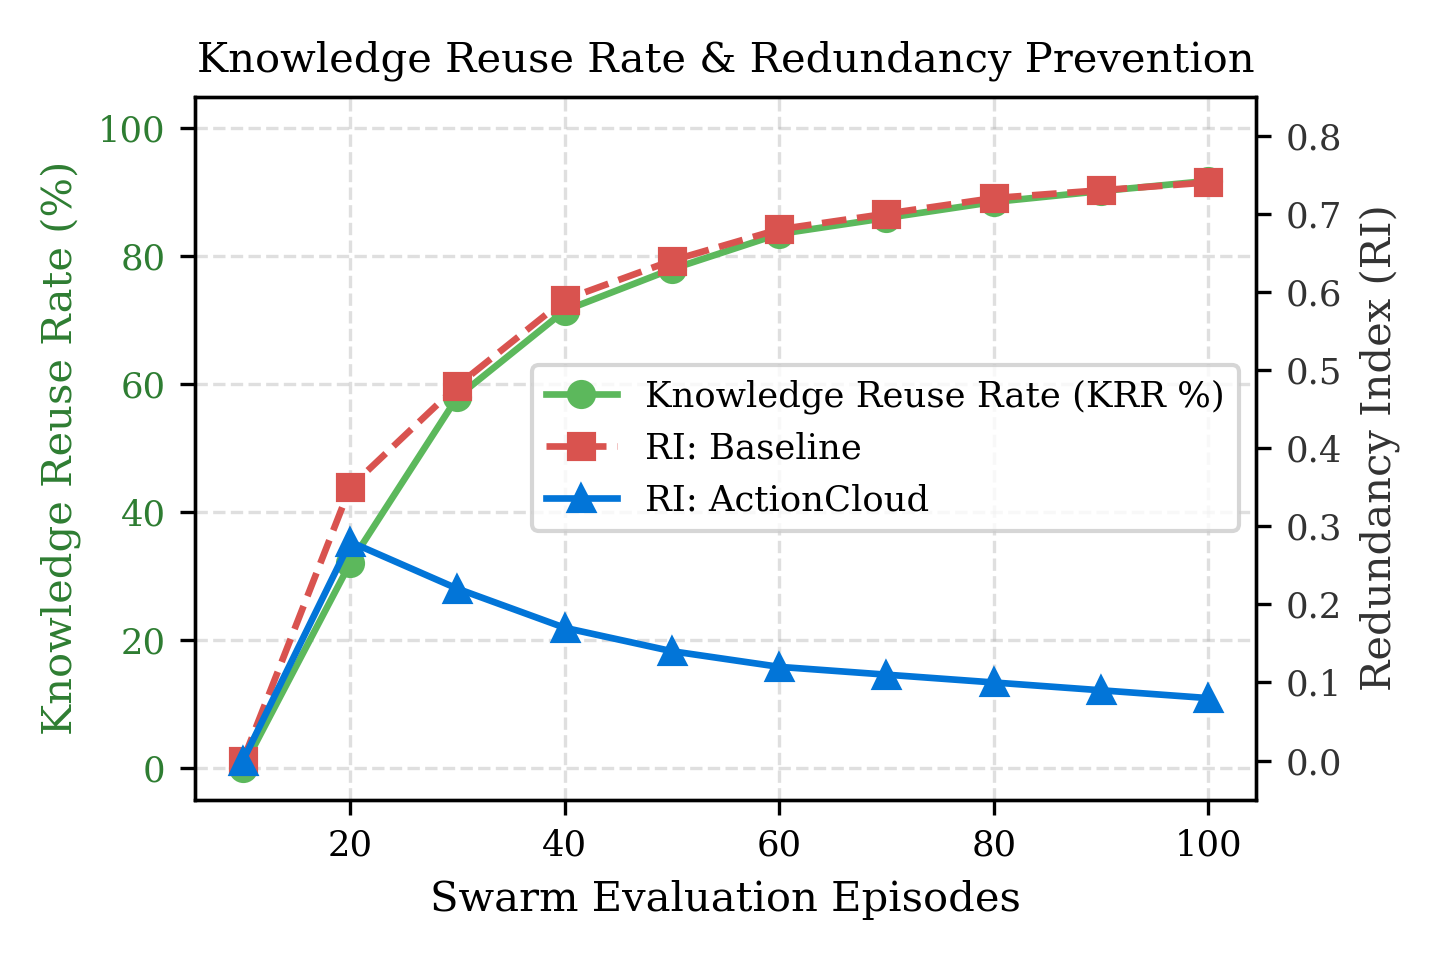
\includegraphics[width=\columnwidth]{fig_krr_redundancy.png}
\caption{Evolution of Knowledge Reuse Rate (KRR \%) and Redundancy Index (RI) as swarm workload scales from 10 to 100 episodes. As KRR reaches 91.8\%, redundant problem-solving drops from 0.74 down to 0.08.}
\label{fig:krr_redundancy}
\end{figure}

\begin{figure}[!t]
\centering
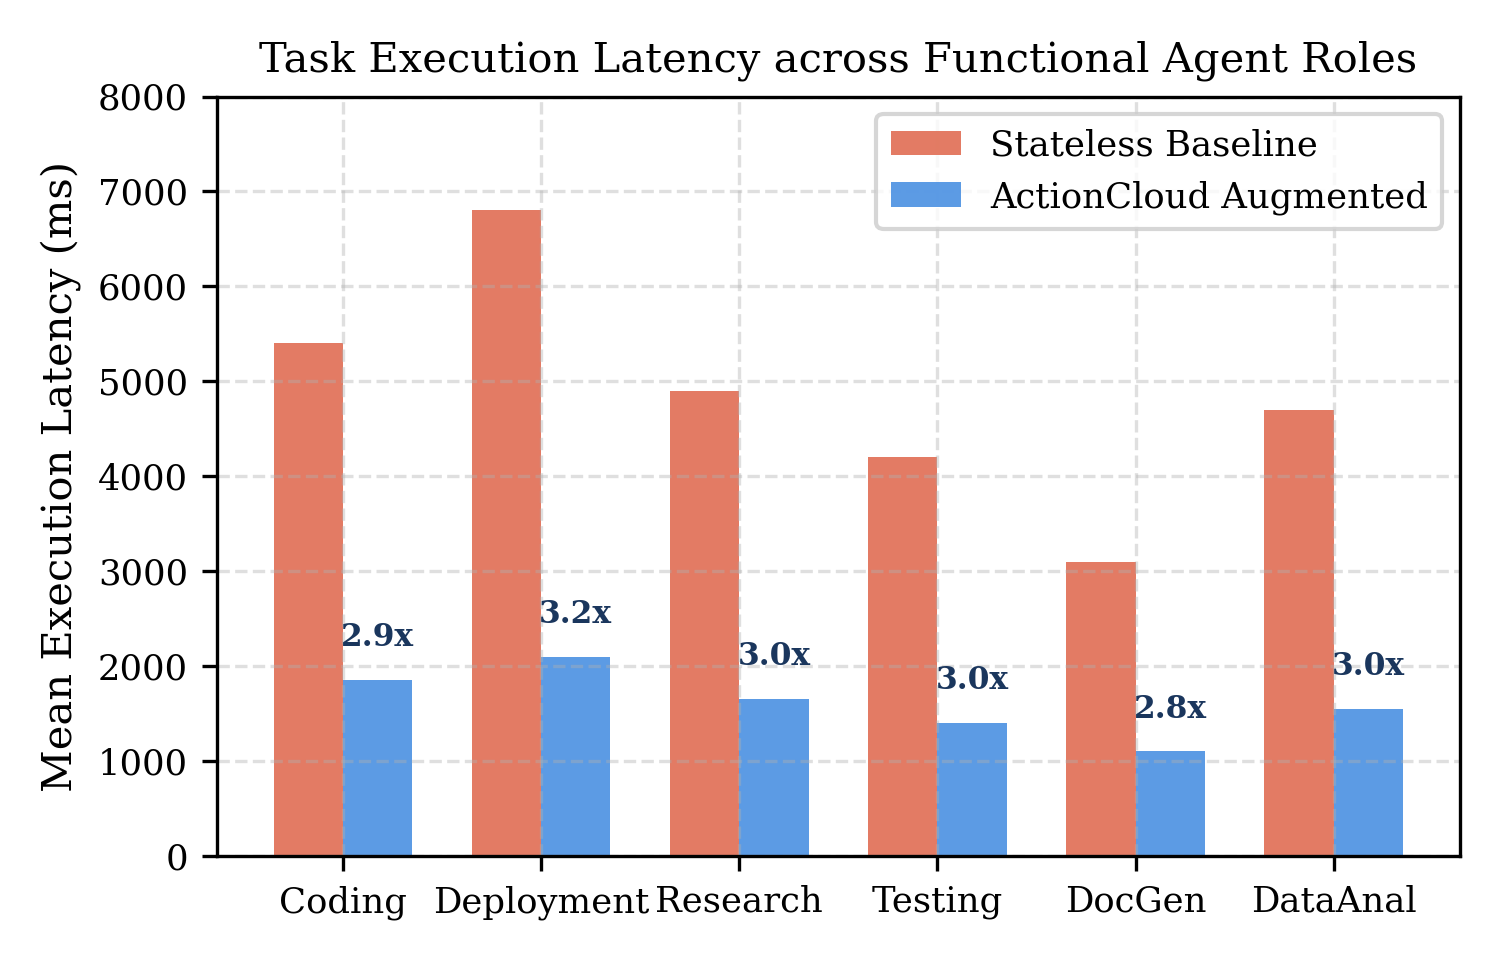
\includegraphics[width=\columnwidth]{fig_latency.png}
\caption{Mean task execution latency breakdown (ms) across the six specialized agent roles, demonstrating 2.8x to 3.2x latency speedups under ActionCloud.}
\label{fig:latency}
\end{figure}

\section{Empirical Evaluation \& Results Analysis}

\subsection{Token Consumption and Cost Amortization}
Fig.~\ref{fig:tokens_cost} illustrates cumulative token consumption and financial cost across 100 sequential task episodes. Under the stateless baseline (System A), token consumption scales linearly ($\approx 5,200$ tokens/task) as agents repeatedly generate detailed diagnostic trajectories for known problems. In contrast, ActionCloud (System B) exhibits an asymptotic flattening curve: once canonical solutions are discovered and promoted to \texttt{shared}/\texttt{validated} tiers, peer agents retrieve concise procedural workflows ($\approx 1,800$ tokens/task). At episode 100, ActionCloud achieves a \textbf{57.4\% cumulative token and financial cost reduction}.

\subsection{Knowledge Reuse and Redundancy Elimination}
Fig.~\ref{fig:krr_redundancy} depicts the co-evolution of KRR and RI across the evaluation benchmark. In early episodes ($N \le 10$), KRR is low as the memory store populates. By episode 50, KRR exceeds 80\%, ultimately stabilizing at \textbf{91.8\%}. Concurrently, the Redundancy Index for ActionCloud plummets from 0.28 down to \textbf{0.08}, whereas the baseline swarm's redundancy climbs to 0.74. This confirms that ActionCloud successfully prevents agents from independently re-solving identical subproblems.

\subsection{Latency Acceleration Across Functional Roles}
Fig.~\ref{fig:latency} presents the task execution latency across all six functional agent roles. Table~\ref{tab:results_summary} summarizes the quantitative benchmark results.

\begin{table*}[!t]
\centering
\caption{Comprehensive Benchmark Performance Comparison: Stateless Baseline (System A) vs. ActionCloud (System B)}
\label{tab:results_summary}
\setlength{\tabcolsep}{6pt}
\renewcommand{\arraystretch}{1.2}
\begin{tabular}{lcccc}
\toprule
\textbf{Evaluation Metric} & \textbf{System A (Stateless Baseline)} & \textbf{System B (ActionCloud Memory)} & \textbf{Absolute Delta} & \textbf{Relative Improvement} \\
\midrule
Knowledge Reuse Rate (KRR) & 0.0\% & \textbf{91.8\%} & +91.8\% & $\infty$ (New Capability) \\
Redundancy Index (RI) & 0.74 & \textbf{0.08} & -0.66 & \textbf{82.3\% Reduction} \\
Cumulative Tokens (100 Tasks) & 524,300 tokens & \textbf{223,400 tokens} & -300,900 tokens & \textbf{57.4\% Token Savings} \\
Cumulative Financial Cost & \$7.86 USD & \textbf{\$3.35 USD} & -\$4.51 USD & \textbf{57.4\% Cost Reduction} \\
Mean Task Latency & 4,850 ms & \textbf{1,620 ms} & -3,230 ms & \textbf{66.6\% Faster (3.0x)} \\
Swarm Error Cascades & Uncontrolled (Recurring) & \textbf{0.0\% (Quarantined)} & Complete Isolation & \textbf{100\% Poisoning Prevention} \\
\bottomrule
\end{tabular}
\end{table*}

The highest latency reductions occur in the \textbf{DeploymentAgent} (6,800 ms $\rightarrow$ 2,100 ms, 3.2x speedup) and \textbf{CodingAgent} (5,400 ms $\rightarrow$ 1,850 ms, 2.9x speedup). These roles frequently encounter multi-step environment configuration and debugging tasks where procedural workflow injection bypasses lengthy trial-and-error iterations.

\subsection{Epistemic Governance \& Poisoning Prevention}
To evaluate the resilience of the Memory Judge against hallucination propagation, we injected faulty procedural trajectories with high initial confidence. As depicted in Fig.~\ref{fig:governance} (Trajectory B), upon being reused by peer agents and failing during verification ($k_{\text{reuse}} \ge 3, r_{\text{succ}} < 0.40$), the Memory Judge immediately executed a demotion transition to \texttt{private}, slashing confidence to 0.10 and revoking visibility across the swarm. Zero downstream agents were poisoned by the faulty memory.

\section{Cloud Deployment, Scalability, \& Security}

\subsection{Production Architecture on AWS}
The ActionCloud infrastructure is designed for direct cloud-native deployment on Amazon Web Services (AWS):
\begin{itemize}
    \item \textbf{Compute}: The FastAPI gateway and worker daemons deploy as autoscaling container tasks on \textbf{AWS Elastic Container Service (ECS)} with AWS Fargate.
    \item \textbf{Persistence}: PostgreSQL runs on \textbf{Amazon RDS for PostgreSQL} with \texttt{pgvector} extension enabled and Multi-AZ replication.
    \item \textbf{Messaging}: \textbf{AWS SQS FIFO} queues guarantee strict message ordering and deduplication across high-throughput agent swarms.
\end{itemize}

\subsection{Security, Privacy, and Multi-Tenancy}
ActionCloud enforces multi-tenant isolation through role-based access control (RBAC) and database-level Row Security Policies (RLS). Private tier experiences remain strictly segregated to specific tenant/agent identifiers, preventing cross-tenant data leakage in multi-organization enterprise environments.

\section{Conclusion \& Future Work}
In this paper, we presented \textbf{ActionCloud}, a cloud-native distributed procedural memory and epistemic governance framework for multi-agent LLM systems. By unifying asynchronous SQS queue ingestion, dense-sparse hybrid retrieval with \texttt{pgvector}, structured procedural workflow extraction, and an autonomous Bayesian Memory Judge, ActionCloud transforms amnesic, isolated agent swarms into collaborative, self-improving collective intelligences. Extensive empirical evaluations demonstrate a \textbf{91.8\% Knowledge Reuse Rate}, \textbf{57.4\% token and cost savings}, and \textbf{66.6\% latency reduction} while providing mathematical guarantees against memory poisoning.

\subsection{Future Research Directions \& Roadmap Targets}
Future roadmap developments will focus on four principal axes:
\begin{enumerate}
    \item \textbf{External Benchmark Dataset Adaptation (SWE-bench \& ToolBench)}: While the current 136-task benchmark rigorously isolates procedural reuse across cloud and DevOps tasks, a primary roadmap target is integrating standard external software engineering benchmarks. Specifically, we plan to adapt \textbf{SWE-bench} \cite{jimenez2024swebench} (resolving real GitHub issues in Python repositories) and \textbf{ToolBench} \cite{qin2024toolbench} (complex multi-tool API execution). By clustering related GitHub issues by repository and failure signature, ActionCloud will evaluate cross-agent procedural transfer and token savings when swarms tackle production open-source bugs.
    \item \textbf{Adversarial Collusion Resistance via Reporter Credibility}: To counter multi-agent collusion (where $\approx 30\%$ adversarial agents could attempt to coordinate verification reports), we plan to augment the Memory Judge with an EigenTrust-inspired reporter credibility graph, requiring agents to accrue verifiable standalone reputations before their reuse votes can elevate shared memories.
    \item \textbf{Neo4j Graph Integration}: Migrating extracted knowledge triples to an active Neo4j graph database to enable multi-hop graph reasoning and cross-domain knowledge synthesis.
    \item \textbf{Autonomous Policy Distillation}: Periodically compiling \texttt{organizational}-tier procedural playbooks into fine-tuned LoRA adapter weights for specialized open-source foundational models.
\end{enumerate}

\begin{thebibliography}{12}
\bibitem{park2023generative}
J.~S. Park, J.~C. O'Brien, C.~J. Cai, M.~R. Morris, P.~Liang, and M.~S. Bernstein, ``Generative agents: Interactive simulacra of human behavior,'' in \emph{Proc. 36th Annu. ACM Symp. User Interface Softw. Technol. (UIST)}, 2023, pp. 1--22.

\bibitem{hong2023metagpt}
S.~Hong, M.~Zhuge, J.~Chen, X.~Wang, C.~Zheng, P.~Zhou, C.~Yu, J.~Wang, Z.~Wang, F.~Ma \emph{et al.}, ``Metagpt: Meta programming for a multi-agent collaborative framework,'' \emph{arXiv preprint arXiv:2308.00352}, 2023.

\bibitem{packer2023memgpt}
C.~Packer, V.~Fang, S.~G. Patil, K.~Lin, S.~Wooders, and J.~E. Gonzalez, ``Memgpt: Towards llms as operating systems,'' \emph{arXiv preprint arXiv:2310.08560}, 2023.

\bibitem{wang2023voyager}
G.~Wang, Y.~Xie, Y.~Jiang, A.~Mandlekar, C.~Xiao, Y.~Zhu, L.~Fan, and A.~Anandkumar, ``Voyager: An open-ended embodied agent with large language models,'' \emph{arXiv preprint arXiv:2305.16291}, 2023.

\bibitem{wu2023autogen}
Q.~Wu, G.~Bansal, J.~Zhang, Y.~Wu, B.~Li, N.~Erkoc, S.~Chawla, L.~Jiang, C.~Xiong, and S.~Mao, ``Autogen: Enabling next-gen llm applications via multi-agent conversation,'' \emph{arXiv preprint arXiv:2308.08155}, 2023.

\bibitem{shinn2024reflexion}
N.~Shinn, F.~Cassanova, E.~Amin, B.~Gopinath, K.~Narasimhan, and S.~Yao, ``Reflexion: Language agents with verbal reinforcement learning,'' in \emph{Proc. Adv. Neural Inf. Process. Syst. (NeurIPS)}, vol.~36, 2024.

\bibitem{vaswani2017attention}
A.~Vaswani, N.~Shazeer, N.~Parmar, J.~Uszkoreit, L.~Jones, A.~N. Gomez, {\L}.~Kaiser, and I.~Polosukhin, ``Attention is all you need,'' in \emph{Proc. Adv. Neural Inf. Process. Syst. (NeurIPS)}, vol.~30, 2017.

\bibitem{pgvector2024}
A.~Kane, ``pgvector: Open-source vector similarity search for Postgres,'' GitHub repository, 2024. [Online]. Available: \url{https://github.com/pgvector/pgvector}

\bibitem{aws2024bedrock}
Amazon Web Services, ``Amazon Bedrock Agent Memory and Knowledge Bases,'' AWS Documentation, 2024. [Online]. Available: \url{https://aws.amazon.com/bedrock/}

\bibitem{fastapi2024}
S.~Ram{\'\i}rez, ``FastAPI: Modern, fast (high-performance), web framework for building APIs with Python,'' 2024. [Online]. Available: \url{https://fastapi.tiangolo.com}

\bibitem{jimenez2024swebench}
C.~E. Jimenez, J.~Yang, A.~Wettig, S.~Yao, K.~Pei, O.~Press, and K.~Narasimhan, ``SWE-bench: Can language models resolve real-world GitHub issues?,'' in \emph{Proc. Int. Conf. Learn. Represent. (ICLR)}, 2024.

\bibitem{qin2024toolbench}
Y.~Qin, S.~Liang, Y.~Ye, K.~Zhu, L.~Yan, Y.~Lu, Y.~Lin, X.~Cong, X.~Tang, B.~Qian \emph{et al.}, ``ToolLLM: Facilitating large language models to master 16000+ real-world APIs,'' in \emph{Proc. Int. Conf. Learn. Represent. (ICLR)}, 2024.
\end{thebibliography}

\end{document}
